% EHMbrAIn project report
% Build:  latexmk -pdf -outdir=build report.tex   (from paper/report/)
% TeXstudio: set the bibliography tool to Biber (Options -> Configure TeXstudio -> Build).
%
% NOTE (public repository): the author remains anonymous in the repository.
% Fill in \author locally for the academic submission; do not commit the name.

\documentclass[11pt,a4paper,oneside]{report}

\usepackage[utf8]{inputenc}
\usepackage[T1]{fontenc}
\usepackage[english]{babel}
\usepackage{lmodern}
\usepackage{microtype}
\usepackage{amsmath,amssymb}
\usepackage{siunitx}
\usepackage{booktabs}
\usepackage{graphicx}
\graphicspath{{figures/}}
\usepackage{csquotes}
\usepackage[style=numeric-comp,sorting=none,backend=bibtex]{biblatex}
\addbibresource{references.bib}
\usepackage[hidelinks]{hyperref}
\usepackage[capitalise]{cleveref}

\newcommand{\code}[1]{\texttt{#1}}

\title{\textbf{EHMbrAIn}\\[2mm]
  \large AI-based versus traditional Engine Health Monitoring:\\
  a gas path analysis testbed on the CFM56-7B with synthetic ground truth}
\author{--- (anonymous in the public repository) ---}
\date{\today\\[2mm]\small Living document: updated at every project milestone.}

\begin{document}

\maketitle
\tableofcontents

\chapter*{Notation and acronyms}
\addcontentsline{toc}{chapter}{Notation and acronyms}

\section*{Acronyms}

\begin{center}\footnotesize
\setlength{\tabcolsep}{4pt}
\begin{tabular}{@{}p{0.10\textwidth}p{0.36\textwidth}p{0.09\textwidth}p{0.36\textwidth}@{}}
  \toprule
  BPR & bypass ratio & LOO & leave-one-out (cross-validation) \\
  CEA & NASA Chemical Equilibrium with Applications & LPC & low-pressure compressor (booster) \\
  CI & continuous integration & LPT & low-pressure turbine \\
  C-MAPSS & NASA turbofan simulation benchmark & MAE & mean absolute error \\
  EEDB & ICAO Engine Emissions Databank & OPR & overall pressure ratio \\
  EGT(M) & exhaust gas temperature (margin) & PC & power code: fraction of reference thrust \\
  EHM & engine health monitoring & PCS & Physics-Consistency Score (ours, C5) \\
  FADEC & full-authority digital engine control & PHM & prognostics and health management \\
  FAR & fuel--air ratio & RMSE & root-mean-square error \\
  FOD & foreign-object damage & RUL & remaining useful life \\
  FPR & false-positive rate & SAC & single annular combustor \\
  GPA & gas path analysis & SHAP & Shapley additive explanations \\
  HPC & high-pressure compressor & SLS & sea-level static \\
  HPT & high-pressure turbine & SVD & singular value decomposition \\
  ICM & influence coefficient matrix & TCDS & type-certificate data sheet \\
  ISA & international standard atmosphere & TSFC & thrust-specific fuel consumption \\
  N1, N2 & low-/high-pressure spool speeds & WLS & weighted least squares \\
  \bottomrule
\end{tabular}
\end{center}

\section*{Symbols}

\begin{center}\footnotesize
\setlength{\tabcolsep}{4pt}
\begin{tabular}{@{}p{0.11\textwidth}p{0.36\textwidth}p{0.11\textwidth}p{0.33\textwidth}@{}}
  \toprule
  $\theta,\ \delta$ & inlet total temperature / pressure ratios to ISA sea level &
    $\mathbf{H}$ & influence coefficient matrix \\
  $\Delta\eta$ & component efficiency deviation [\%] &
    $\mathbf{Q},\ \mathbf{R}$ & process / measurement noise covariance \\
  $\Delta\Gamma$ & component flow-capacity deviation [\%] &
    $\mathbf{P}_0,\ \lambda$ & prior shape / strength of the WLS regularization \\
  $\mathbf{x}$ & health-parameter vector (10 components) &
    $N1_c$ & corrected fan speed $N1/\sqrt{\theta}$ \\
  $\Delta\mathbf{z}$ & measurement deviations from baseline &
    $T_{t4}$ & combustor-exit total temperature \\
  $W_f,\ F_n$ & fuel flow, net thrust &
    $\Delta T_{\mathrm{ISA}}$ (dTs) & ambient offset from the ISA day \\
  \bottomrule
\end{tabular}
\end{center}

\paragraph{Reading order.} Every technical term is defined at first use;
\cref{ch:background} builds the engine and GPA foundations,
\cref{sec:ai-toolbox} the machine-learning toolbox. The hypotheses table
(\cref{tab:hypotheses}) can be read superficially on a first pass and revisited
after those two stops.

\chapter{Introduction}
\label{ch:introduction}

\begin{quote}\itshape
This chapter in brief: jet engines degrade invisibly, airlines monitor them through a handful
of measurements, and two schools of methods compete to interpret those measurements. This
project builds a level playing field to compare them. If you are new to the field, skim the
hypotheses table on first read and return to it after \cref{ch:background}.
\end{quote}

\keyidea{The field compares AI against weakly-implemented traditional baselines. The only honest comparison gives both families \emph{identical} data, metrics, splits and tuning budget; everything in this document follows from insisting on that symmetry.}


\section{Motivation}

A commercial jet engine degrades from its very first flight. Dust and pollution stick to
compressor blades, hot-section parts creep and oxidize, tip clearances open up, seals wear.
The airline cannot see any of this directly ---the engine stays on the wing for years--- so it
watches the engine's \emph{symptoms} instead: the temperatures, pressures, shaft speeds and fuel
flow recorded on every flight. The discipline that turns those symptoms into maintenance
decisions is called \emph{Engine Health Monitoring} (EHM). The stakes are large: a single shop
visit for an engine overhaul costs millions of dollars, and an unscheduled engine removal
disrupts an entire fleet schedule.

The classical analytical core of EHM, in use since the 1970s, is \emph{Gas Path Analysis}
(GPA)~\cite{Urban1975}. The idea: each physical fault (a dirty compressor, an eroded turbine)
leaves a characteristic fingerprint on the measured parameters; by inverting a thermodynamic
model of the engine, one can estimate \emph{which} component has deteriorated and \emph{by how
much} from the measurements alone. Around GPA the industry built a mature toolbox ---baseline
models, exponential trend smoothing, Kalman filters, expert fault-isolation rules%
~\cite{Volponi2014}--- which this project collectively calls \emph{traditional EHM}.

Over the last decade, machine learning (ML) has produced striking results in the adjacent research
field of prognostics: predicting the \emph{Remaining Useful Life} (RUL) of an engine, i.e.\ how
many flights remain before it must come off the wing, mostly on synthetic benchmark datasets
such as NASA's C-MAPSS~\cite{Saxena2008} and N-CMAPSS~\cite{AriasChao2021}. Yet the literature
has a structural weakness: \textbf{AI methods are almost never compared against a traditional
pipeline implemented with equal care}, on the same data, with the same metrics and the same
tuning effort. The result is a stream of comparisons against straw men, which makes it
impossible to know what AI actually contributes, under which conditions, and at what cost.

\section{Objective}

This project builds a reproducible testbed in which both EHM families ---traditional and
AI-based--- observe \emph{exactly the same data} from a synthetic fleet of CFM56-7B26 turbofans
and are scored with \emph{exactly the same metrics}. The methodological key is that the
synthetic data carries \textbf{complete ground truth}: the true health state of every engine
component (its efficiency and flow-capacity deviations, defined in \cref{sec:gpa}) at every
flight. With real airline data this is impossible ---nobody knows the true internal state of an
engine on the wing--- but with synthetic data one can measure not only whether a method detects
or predicts well, but whether it \emph{attributes the damage to the correct component}. That
attribution question is precisely where traditional GPA is weakest (the \emph{smearing}
phenomenon, \cref{sec:gpa}) and where AI is least transparent (the black-box problem).

\paragraph{Audience and register.} This document is a research work aimed at two readers at
once: the engineering organization deciding whether and how to integrate AI into its engine
health monitoring practice, and the researcher looking for a rigorous, reproducible
benchmark at the knowledge frontier. That dual audience sets the register: every method is
pushed to publishable rigor (pre-registration, statistical tests, audited datasets), and
every concept is introduced without assuming prior specialization --- chapter briefs, worked
numeric examples and a notation front-matter keep the document self-contained. Advancing the
frontier and being readable are treated as the same job, not competing ones.

Since neither a performance model of the engine nor degradation data were available to the
project, both are built from scratch: a thermodynamic ``digital twin'' of the CFM56-7B26 in
pyCycle~\cite{Hendricks2019}, calibrated against certified public data (\cref{ch:model}), and a
fleet degradation generator with physically derived fault signatures (\cref{ch:fleet}).

\section{Hypotheses}
\label{sec:hypotheses}

Each hypothesis is formalized with quantitative thresholds \emph{before} any test-set result is
seen (the pre-registration protocol of \cref{sec:safeguards}). All are tested with a Wilcoxon
signed-rank test paired by engine, Holm correction for multiple comparisons
($\alpha = 0.05$), and BCa bootstrap confidence intervals. In plain words: for every comparison
we check that the improvement is statistically significant, not a fluke of one lucky engine.
The table below necessarily uses terms defined later ---the GPA quantities in
\cref{ch:background}, the machine-learning methods in \cref{sec:ai-toolbox}, every metric in
the metrics section of \cref{ch:methodology}, and all acronyms in the notation chapter--- so
it is meant to be skimmed now and revisited after those stops.

\begin{table}[htbp]
  \centering\small
  \caption{Project hypotheses and their confirmation criteria.}
  \label{tab:hypotheses}
  \begin{tabular}{p{0.04\textwidth}p{0.36\textwidth}p{0.50\textwidth}}
    \toprule
    ID & Hypothesis & Confirmation criterion \\
    \midrule
    H1 & AI detects faults earlier and with fewer false alarms than trend monitoring &
      median lead time $\geq +20$\,\% and false-positive rate $\leq 0.5\times$ versus
      trending, at a fixed recall of $0.9$; $p<0.05$ \\
    H2 & AI isolates faults with overlapping signatures better &
      $+10$ percentage points of isolation accuracy on the ``confusable'' subset (fault
      signatures less than $15^{\circ}$ apart in the influence-matrix space) versus
      weighted-least-squares GPA; $p<0.05$ \\
    H3 & AI predicts RUL better &
      simultaneous improvement in RMSE and in the asymmetric NASA PHM08 score; $p<0.05$ \\
    H4 & The physics-informed hybrid dominates when data is scarce &
      RUL RMSE $\leq$ pure AI with 100\,\% of the training data and strictly better with
      10\,\% and 25\,\%; $p<0.05$ \\
    H5 & Conformal intervals are better calibrated than the Kalman covariance &
      smaller $|$empirical coverage $-$ 0.9$|$ with mean interval width no worse than
      $+20$\,\% \\
    \bottomrule
  \end{tabular}
\end{table}

Refuting any hypothesis is itself a publishable result: pre-registration is what makes the
refutation credible. Reformulating hypotheses after the repository tag \code{prereg-v1} is
forbidden. One operationalization was refined \emph{at} the freeze, before any test-set run
and disclosed in the frozen document: H1's ``fixed recall $0.9$'' proved unreachable at the
v1.1 fault magnitudes, so its operating point was redefined per family under a false-alarm
budget (\cref{sec:res-h1}). Changing an operating definition at freeze time, on the record,
is legitimate; changing a threshold after seeing the answer is what the tag forbids.

\section{Contributions}
\label{sec:contributions}

In plain terms first, before the technical names: the project builds a realistic test dataset
with hidden answers no real fleet can provide (C1), runs a scrupulously fair contest between
the two method families (C2), and from it delivers a physics-informed hybrid (C3), calibrated
uncertainty (C4), a physics-anchored explainability score (C5), a sensor-and-data trade map
(C6), an external reality check (C7), and --- the furthest reach --- two per-engine
certificates, proven against the truth, of what a diagnosis can honestly know (C8) and how
much of an engine's future its present can reveal (C9). Each item below names
the technique; every term is defined where it is first used, so this list is a preview, not a
prerequisite.

\begin{enumerate}
  \item[\textbf{C1.}] \textbf{SynCFM56}: the first public synthetic GPA dataset for a specific
    commercial engine (CFM56-7B26), with per-flight health-parameter ground truth and an
    ACARS-style snapshot format (one takeoff report and one cruise report per flight, the way
    real airline EHM data actually arrives), more realistic than the continuous time series of
    C-MAPSS.
  \item[\textbf{C2.}] A head-to-head comparison under a \textbf{pre-registered protocol} with a
    symmetric tuning budget (the same number of Optuna trials) for both families.
  \item[\textbf{C3.}] A physics-informed hybrid with three separately ablated mechanisms:
    residual features against the digital twin, physically constrained loss functions, and
    GPA$\rightarrow$ML stacking.
  \item[\textbf{C4.}] Compared uncertainty quantification: conformal-prediction RUL intervals
    versus the Kalman filter covariance.
  \item[\textbf{C5.}] The \textbf{Physics-Consistency Score (PCS)}: a new explainability metric
    that projects SHAP attributions into the physical health-parameter space through the
    influence coefficient matrix.
  \item[\textbf{C6.}] A determinability map: a sensors $\times$ noise $\times$ data-size
    ablation showing \emph{when} each approach wins --- the sensor axis throughout
    (\cref{sec:icm,ch:gpa-practice}), the data-size axis in the H4 ablation
    (\cref{sec:ai-hybrid}), and the noise axis swept from half to four times nominal sensor
    quality in \cref{sec:noise-sweep}.
  \item[\textbf{C7.}] Sim-to-real validation: the full methodology is re-run on N-CMAPSS to
    check that the method ranking is not an artifact of our own simulator.
  \item[\textbf{C8.}] \textbf{The earned-confidence certificate} (\cref{ch:breakthrough}): a
    per-engine, history-resolved identifiability guarantee for gas-path diagnosis --- and,
    uniquely, a \emph{proof against ground truth} that it is honest ($\rho = 0.70$ between
    certified precision and actual error). It states exactly which health directions an
    engine's data lets one conclude, and doubles as a sensor-acquisition instrument
    (predicting that station probes rescue HPC efficiency $45\times$). The validation is one
    only a synthetic-truth benchmark can perform.
  \item[\textbf{C9.}] \textbf{The prognostic floor} (\cref{sec:bt-prognostic-floor}): the
    predictive counterpart of C8. By conditioning on each engine's \emph{true} current health
    state it measures, against ground truth, the aleatoric floor on remaining-life error --- the
    RMSE no method can beat. It shows $87\,\%$ of mid-life RUL uncertainty is irreducible, yet a
    $4\times$ reducible gap opens late in life, telling an operator \emph{where} a better
    prognostic is worth building and where the future is simply unknowable.
\end{enumerate}

\section{Document structure}

The document follows the work in order, and a reader can stop wherever their interest ends.
\Cref{ch:background} builds the foundations from zero: how a turbofan works, what is measured
on the wing, and the mathematics of gas-path diagnosis --- no prior knowledge assumed.
\Cref{ch:methodology} lays out the testbed and the fairness safeguards that make the
comparison trustworthy. The next chapters build the ingredients: the thermodynamic twin
of the engine (\cref{ch:model}), the classical gas-path diagnosis measured end to end on that
twin --- the quantitative floor everything later is compared against
(\cref{ch:gpa-practice}) --- what the data \emph{is} and where it comes from
(\cref{ch:data}), and the synthetic fleet generated from it (\cref{ch:fleet}). The two EHM
families are then implemented and measured --- traditional (\cref{ch:trad}) and AI
(\cref{ch:ai}) --- and adjudicated head to head under the pre-registered protocol
(\cref{ch:results}), with five real engines telling the story in operations language
(\cref{ch:cases}).

The remaining chapters push past the main study. \Cref{ch:tomography} asks whether more
observability can be bought without new hardware; \cref{ch:overcoming} turns each declared
limitation into its own experiment; \cref{ch:breakthrough} is the project's furthest reach,
the ground-truth-validated certificate; and \cref{ch:economics} asks, cautiously, what any of
it is worth. \Cref{ch:conclusions} closes. The appendices hold the decision register (every
choice and its justification), the dated milestone log, and a plain-language deep dive on how
each machine-learning method works (\cref{ch:ml-appendix}).

\chapter{Background}
\label{ch:background}

This chapter assumes no prior knowledge of gas turbines. It introduces the engine, the
measurements available in service, the mathematics of gas path diagnosis, and the physics of
degradation ---everything needed to follow the rest of the document.

\section{How a two-spool turbofan works}
\label{sec:turbofan}

A turbofan produces thrust by accelerating air backwards. Air enters through the \emph{fan} (the
large visible rotor); most of it ---the \emph{bypass} stream--- goes around the core and exits
through the bypass nozzle, producing the majority of the thrust. The rest enters the \emph{core}:
it is compressed by a low-pressure compressor (the \emph{booster}) and a high-pressure
compressor (HPC), heated by burning fuel in the \emph{combustor}, and expanded through a
high-pressure turbine (HPT) and a low-pressure turbine (LPT) that extract the work needed to
drive the compressors, before leaving through the core nozzle.

The machine is arranged in two mechanically independent \emph{spools} (concentric shafts):
\begin{itemize}
  \item the \textbf{low-pressure (LP) spool}: fan + booster driven by the LPT, rotating at speed
    \textbf{N1};
  \item the \textbf{high-pressure (HP) spool}: HPC driven by the HPT, rotating at speed
    \textbf{N2}.
\end{itemize}
The ratio of bypass to core mass flow is the \emph{bypass ratio} (BPR); the ratio of compressor
exit pressure to inlet pressure is the \emph{overall pressure ratio} (OPR). Higher BPR and OPR
generally mean better fuel efficiency, measured as \emph{thrust-specific fuel consumption}
(TSFC): fuel flow per unit of thrust.

\section{The subject engine: CFM56-7B26}
\label{sec:engine}

The CFM56-7B (CFM International, a Safran--GE joint venture) powers the Boeing 737NG family and
is one of the most widely operated commercial engines in history, which guarantees abundant
public type data. The \textbf{-7B26} variant (\SI{117}{\kilo\newton} takeoff thrust, Boeing
737-800) is chosen as the most common one. Its type-certificate data sheet (TCDS EASA E.004,
issue~07~\cite{EASA2023}) describes: a single-stage fan, 3-stage booster, 9-stage HPC, annular
combustor, single-stage HPT and 4-stage LPT, governed by a dual-channel FADEC (a full-authority
digital engine control ---the computer that meters fuel). The pilot-facing thrust-setting
parameter is N1, not engine pressure ratio.

\begin{table}[htbp]
  \centering\small
  \caption{Certified CFM56-7B26 data used as the calibration contract. Sources: TCDS EASA E.004
  issue~07~\cite{EASA2023} and the ICAO Engine Emissions Databank, edition 03/2026, UID
  3CM033~\cite{ICAO2026}.}
  \label{tab:tcds}
  \begin{tabular}{llll}
    \toprule
    Quantity & Value & Source & Status \\
    \midrule
    Takeoff thrust & \SI{11699}{\deca\newton} (= \SI{116.99}{\kilo\newton}) & TCDS & verified \\
    Maximum continuous thrust & \SI{11521}{\deca\newton} & TCDS & verified \\
    N1 redline (104\,\%) & \SI{5382}{rpm} $\Rightarrow$ 100\,\% = \SI{5175}{rpm} & TCDS & verified \\
    N2 redline (105\,\%) & \SI{15183}{rpm} $\Rightarrow$ 100\,\% = \SI{14460}{rpm} & TCDS & verified \\
    Max.\ EGT, takeoff / continuous & \SI{950}{\degreeCelsius} / \SI{925}{\degreeCelsius} (displayed) & TCDS & verified \\
    Dry weight & \SI{2386}{\kilo\gram} & TCDS & verified \\
    Bypass ratio & 5.1 & EEDB & verified \\
    Pressure ratio (sea-level static, rated) & 27.61 & EEDB & verified \\
    Fuel flow at 100/85/30/7\,\% $F_{00}$ & 1.221 / 0.999 / 0.338 / 0.113 \si{\kilo\gram\per\second} & EEDB & verified \\
    \bottomrule
  \end{tabular}
\end{table}

Two subtleties from the TCDS matter for modeling and are frequently overlooked:
\begin{itemize}
  \item The certified \emph{exhaust gas temperature} (EGT) ---the single most important health
    indicator, because it rises as the engine deteriorates--- is measured at station
    \textbf{T49.5} (the stage-2 LPT nozzle), \emph{not} at the HPT exit. Moreover, the
    \emph{displayed} cockpit value adds a ``shunt'' function of $+\SI{30}{\degreeCelsius}$ (for
    single-annular-combustor engines, active above \SI{8500}{rpm} N2) plus a model-dependent
    ``trim'' (zero for the -7B26).
  \item Air bleed limits (air extracted from the compressor for the aircraft's cabin and
    anti-ice systems) are tabulated per extraction stage and shaft speed; at rated speed the
    9th-stage bleed is capped at 7\,\% of core flow.
\end{itemize}

\section{What is measured, and why parameters must be corrected}
\label{sec:stations}

Engine locations are numbered per the SAE ARP755A standard~\cite{SAE755}: station 2 is the fan
inlet, 21 the fan exit, 25 the HPC inlet, 3 the HPC exit, 4 the combustor exit, 45 the HPT
exit, and 5 the LPT exit. The measurements available in airline service (the ``cockpit set'')
are N1, N2, EGT and fuel flow $W_f$; some installations add pressures and temperatures at
stations 25 and 3.

A raw measurement is meaningless on its own because it depends on the day: the same healthy
engine reads a higher EGT on a hot day at a high-altitude airport than on a cold day at sea
level. To compare flights, measurements are \emph{corrected} to standard sea-level conditions
using $\theta = T_{t2}/\SI{288.15}{\kelvin}$ and $\delta = P_{t2}/\SI{101.325}{\kilo\pascal}$
(the ratios of inlet total temperature and pressure to their standard-day values):
\begin{equation}
  N_{\mathrm{corr}} = \frac{N}{\sqrt{\theta}}, \qquad
  W_{f,\mathrm{corr}} = \frac{W_f}{\delta\,\theta^{a}}, \qquad
  \mathrm{EGT}_{\mathrm{corr}} = \frac{\mathrm{EGT}}{\theta}.
\end{equation}
The exponent $a$ (typically 0.5--0.7) is often copied from generic tables; here it will instead
be fitted by regression on sweeps of our own thermodynamic model, removing a classical source
of systematic baseline error.

\section{Gas Path Analysis}
\label{sec:gpa}

\subsection{Health parameters}

GPA describes the internal state of the engine with two numbers per turbomachine: the deviation
of its \emph{isentropic efficiency} $\Delta\eta$ (how much of the ideal work it actually
achieves ---dirt and wear reduce it) and the deviation of its \emph{flow capacity}
$\Delta\Gamma$ (how much corrected flow it swallows at a given speed ---fouling reduces it in
compressors; turbine erosion, which opens the effective nozzle area, increases it). With five
turbomachines (fan, booster, HPC, HPT, LPT) the health state is the 10-component vector
\begin{equation}
  \mathbf{x} = \left[\Delta\eta_{\mathrm{fan}}, \Delta\Gamma_{\mathrm{fan}},
  \Delta\eta_{\mathrm{LPC}}, \Delta\Gamma_{\mathrm{LPC}},
  \Delta\eta_{\mathrm{HPC}}, \Delta\Gamma_{\mathrm{HPC}},
  \Delta\eta_{\mathrm{HPT}}, \Delta\Gamma_{\mathrm{HPT}},
  \Delta\eta_{\mathrm{LPT}}, \Delta\Gamma_{\mathrm{LPT}}\right]^{\mathsf T},
\end{equation}
expressed in percent relative to a new engine. $\mathbf{x}$ is what maintenance actually wants
to know, and it is not directly measurable on the wing.

\subsection{The linear model}

What \emph{is} measurable are deviations $\Delta\mathbf{z}$ of the corrected parameters from a
\emph{baseline} (the value a new engine would show at the same operating condition
$\mathbf{u}$: altitude, Mach number, N1 setting, ambient temperature deviation, bleed status).
For the small deviations typical of in-service deterioration, measurement and health deviations
are related linearly:
\begin{equation}
  \Delta\mathbf{z} = \mathbf{H}(\mathbf{u})\,\mathbf{x} + \mathbf{S}\,\mathbf{b} + \mathbf{v},
  \qquad \mathbf{v}\sim\mathcal{N}(\mathbf{0},\mathbf{R}),
  \label{eq:gpa-linear}
\end{equation}
where $\mathbf{H}$ is the \emph{influence coefficient matrix} (ICM) ---the Jacobian
$\partial\mathbf{z}/\partial\mathbf{x}$, i.e.\ a table of ``if the HPT loses 1\,\% efficiency,
EGT rises by this much and fuel flow by that much''--- computed by finite differences on the
thermodynamic model at the operating condition $\mathbf{u}$; $\mathbf{b}$ collects sensor
biases; and $\mathbf{v}$ is measurement noise with covariance $\mathbf{R}$.

\subsection{Estimation, and why it is hard}

Inverting \cref{eq:gpa-linear} is an ill-posed problem. With 4 cockpit measurements and 10
unknowns the system is underdetermined ($\operatorname{rank}(\mathbf{H})\leq 4$): infinitely
many health states explain the same measurements. The weighted-least-squares (WLS) answer
regularizes the inversion with prior knowledge of plausible deterioration:
\begin{equation}
  \hat{\mathbf{x}} = \left(\mathbf{H}^{\mathsf T}\mathbf{R}^{-1}\mathbf{H}
  + \lambda\,\mathbf{P}_0^{-1}\right)^{-1}\mathbf{H}^{\mathsf T}\mathbf{R}^{-1}\Delta\mathbf{z},
  \label{eq:wls}
\end{equation}
where the two regularization pieces play distinct roles: $\mathbf{P}_0$ (a diagonal matrix of
expected deterioration magnitudes squared) sets the \emph{shape} of the prior --- which
parameters are allowed to move more --- while the scalar $\lambda$ sets its \emph{strength},
trading fidelity to the measurements against fidelity to the prior. $\lambda$ is a tuning knob
of the traditional pipeline and receives the same optimization budget as the AI's
hyperparameters (\cref{sec:safeguards}).

Because deterioration evolves slowly over thousands of flights, tracking it as a
\emph{random walk} with a Kalman filter improves on flight-by-flight estimation. The Kalman
filter is a recursive estimator that blends the previous health estimate with each new
measurement, weighting each by its uncertainty:
\begin{equation}
  \mathbf{x}_k = \mathbf{x}_{k-1} + \mathbf{w}_k, \quad
  \mathbf{w}\sim\mathcal{N}(\mathbf{0},\mathbf{Q});
  \qquad
  \mathbf{z}_k = \mathbf{H}(\mathbf{u}_k)\,\mathbf{x}_k + \mathbf{v}_k,
  \label{eq:kalman}
\end{equation}
with process noise $\mathbf{Q}$ calibrated to realistic degradation rates and the state
optionally augmented with sensor biases~\cite{Volponi2014}. At recorded compressor-wash events
the recoverable part of the state is reset.

\subsection{Smearing}

When $\mathbf{H}$ is ill-conditioned ---some fault signatures are nearly parallel--- noise makes
the estimator distribute a fault that is physically concentrated in one component across
several: the \emph{smearing} phenomenon, the classical weakness of linear GPA~\cite{Li2002}.
A singular-value decomposition (SVD) of the ICM quantifies this weakness (rank, condition
number, angles between fault signatures) and defines the ``confusable'' subset used by
hypothesis H2: fault pairs whose signatures are less than $15^{\circ}$ apart.

\section{The physics of degradation}
\label{sec:degradation}

\begin{table}[htbp]
  \centering\small
  \caption{Degradation mechanisms modeled in this project and their typical effects, per the
  literature~\cite{Diakunchak1992,Kurz2012}.}
  \label{tab:degradation}
  \begin{tabular}{p{3.0cm}p{2.2cm}p{3.8cm}p{2.6cm}p{1.6cm}}
    \toprule
    Mechanism & Component & Typical effect & Time profile & Recoverable \\
    \midrule
    Fouling (dirt buildup) & fan/LPC/HPC & $\Delta\Gamma$ $-1$\ldots$-4$\,\%; $\Delta\eta$ $-0.5$\ldots$-2.5$\,\% & saturating exponential & wash recovers 30--70\,\% \\
    Erosion & compressors & $\Delta\eta$ $-0.5$\ldots$-1.5$\,\% & slow linear & no \\
    Tip-clearance opening & HPC/HPT & $\Delta\eta$ $-0.5$\ldots$-1.5$\,\% & fast initially, then slow & no \\
    Hot-section deterioration & HPT & $\Delta\eta$ $-1$\ldots$-3$\,\%; $\Delta\Gamma$ $+1$\ldots$+2$\,\% & linear/accelerating & no \\
    Foreign-object damage (FOD) & fan/HPC & step $\Delta\eta$ $-0.5$\ldots$-2$\,\% & step (Poisson arrivals) & no \\
    Sensor drift & any probe & e.g.\ EGT $+1$\ldots$+5$~\si{\degreeCelsius} per 1000 cycles & ramp & recalibration \\
    \bottomrule
  \end{tabular}
\end{table}

The aggregate observable effect is the erosion of the \emph{EGT margin}: the distance between
the EGT reached on a hot-day takeoff and its certified limit. A new engine has
\SI{70}{}--\SI{100}{\degreeCelsius} of margin; when the margin reaches zero the engine can no
longer legally produce rated takeoff thrust on a hot day and must come off the wing. Its
characteristic pattern over an engine's life ---fast early loss, slower steady erosion, sawtooth
recoveries at each compressor wash--- is what the fleet generator of phase F2 must reproduce.
\Cref{tab:degradation} summarizes the mechanisms, their signatures and their time profiles; its
magnitudes parameterize that generator.

\chapter{Methodology and testbed architecture}
\label{ch:methodology}

\section{Overall architecture}

The testbed is organized in six chained phases, each closed by a milestone (\emph{gate}) with a
measurable acceptance criterion:

\begin{enumerate}
  \item[\textbf{F1.}] \textbf{Thermodynamic twin} of the CFM56-7B26 in pyCycle: design point,
    off-design behavior, baseline decks over the flight envelope (pre-computed tables of what a
    healthy engine reads at every operating condition) and the influence coefficient matrix.
    Gate H1: error $\leq 3$\,\% against certified data at the anchor points.
  \item[\textbf{F2.}] \textbf{Synthetic fleet generator} (SynCFM56): per-mechanism health
    trajectories, a hierarchical fleet of $\sim$100 engines run to failure, a sensor model
    (noise, bias, quantization, missing data) and ACARS-style snapshots with ground truth.
    Gate H2: dataset audited for realism and difficulty, no leakage between data splits, and a
    written datasheet.
  \item[\textbf{F3.}] \textbf{Traditional EHM} reference: baselines and smoothed deviations,
    trend monitoring with persistence rules, WLS GPA (\cref{eq:wls}), Kalman GPA
    (\cref{eq:kalman}), expert-rule fault isolation, and RUL by robust extrapolation of the EGT
    margin. Gate H3: full metrics on the test set.
  \item[\textbf{F4.}] \textbf{AI-based EHM}: anomaly detection (autoencoders, Isolation
    Forest), multi-class fault diagnosis (gradient boosting, neural networks), RUL prognosis
    (LSTM/TCN/Transformer sequence models), the physics-informed hybrid, conformal uncertainty
    and physical explainability (PCS). Gate H4.
  \item[\textbf{F5.}] \textbf{Pre-registered comparative evaluation}: common metrics,
    statistical tests, ablations, and sim-to-real validation on N-CMAPSS. Gate H5.
  \item[\textbf{F6.}] Case studies, interactive dashboard, and final writing. Gate H6.
\end{enumerate}

\section{Methodological safeguards}
\label{sec:safeguards}

The credibility of an AI-versus-traditional comparison depends on eliminating the biases that
plague the literature. Four safeguards are adopted:

\begin{description}
  \item[Pre-registration.] Hypotheses (\cref{tab:hypotheses}), metrics, data splits (with file
    hashes), statistical tests and the stopping rule are frozen in the repository under a git
    tag (\code{prereg-v1}) \emph{before} the test set is evaluated. This borrows a standard
    practice from medicine: you state what would convince you before looking at the answer, so
    you cannot move the goalposts afterwards.
  \item[Symmetric tuning budget.] Every method has knobs. The traditional pipeline's
    (alert thresholds, regularization $\lambda$, Kalman $\mathbf{Q}$, smoothing windows) and
    each AI family's hyperparameters are tuned with the \emph{same number} of automated search
    trials (Optuna), using only the training and validation engines.
  \item[Split by engine.] The fleet is divided 70/10/20 engines into training, validation and
    test sets, and no engine ever appears in two sets. Splitting by flight instead of by engine
    ---a common mistake--- would let a model memorize an engine's individual quirks and score
    unrealistically well. An automated leakage check runs in continuous integration.
  \item[A strong baseline.] The traditional pipeline is implemented with the same care as the
    AI, every expert rule documented with its physical justification; smearing is
    \emph{measured} against ground truth, not assumed.
\end{description}

\section{Reproducibility and infrastructure}
\label{sec:reproducibility}

The entire project is a public
repository\footnote{\url{https://github.com/cedarcreeks/EHMbrAIn}} with a reproducible
environment: Python~3.11 managed with \code{uv} and a fully pinned dependency lockfile;
pyCycle~4.4 on OpenMDAO~\cite{Gray2019}; declarative YAML configuration; and automated tests
(pytest) executed by continuous integration ---a service that re-runs the whole test suite on
every change, so a regression cannot land silently. Data and experiments of later phases will
be versioned with DVC and MLflow respectively.

Three concrete decisions illustrate the intended standard of rigor:

\begin{itemize}
  \item \textbf{A versioned calibration contract.} The model's numerical targets
    (\cref{tab:tcds}) live in a single file (\code{conf/cfm56\_7b\_targets.yaml}) carrying
    value, tolerance, source and status (\code{VERIFIED}/\code{TO\_VERIFY}) per entry. Both the
    model runners and the tests read that file: changing a target is a visible version-control
    event, never a silent edit.
  \item \textbf{Dependency canary tests.} During environment setup, an incompatibility between
    pyCycle~4.4 and numpy~$\geq 2$ was discovered (a failure inside the tabular thermodynamics
    package). The fix pins \code{numpy<2}, and a smoke test that runs a complete engine cycle
    executes on every CI run, so any future dependency upgrade that breaks the solver fails
    loudly and immediately.
  \item \textbf{Auto-generated evidence.} Every result figure and table in this document is
    produced by a script (\code{scripts/make\_report\_assets.py}) that solves the model and
    writes the PDFs, the \LaTeX{} table files (\code{paper/report/tables/*.tex}) and a
    provenance file (\code{assets.json}). No result number is ever copied by hand.
\end{itemize}

\section{Comparison metrics}

Both families are scored with identical metrics. For detection: lead time (how many flights
before the ground-truth event the method raises a sustained alert), false alarms per thousand
flights, F1 and precision-recall AUC. For isolation: top-1/top-2 accuracy, macro-F1, a
\emph{smearing index} (the fraction of $\|\hat{\mathbf{x}}\|_1$ assigned to healthy components)
and the PCS. For health estimation: RMSE of $\hat{\mathbf{x}}$ against ground truth. For RUL:
RMSE, MAE, the NASA PHM08 score
\begin{equation}
  S=\sum_i s_i,\qquad
  s_i = \begin{cases} e^{-d_i/13}-1 & d_i<0\\ e^{d_i/10}-1 & d_i\geq 0\end{cases},
  \qquad d_i = \widehat{\mathrm{RUL}}_i - \mathrm{RUL}_i,
\end{equation}
which penalizes late predictions more than early ones (a late removal risks an in-flight
shutdown; an early one merely wastes some life), plus $\alpha$--$\lambda$ accuracy and the
prognostic horizon. For uncertainty: empirical versus nominal interval coverage and mean
interval width.

\chapter{Thermodynamic twin of the CFM56-7B26}
\label{ch:model}

This chapter documents the completed part of phase F1: the CFM56-7B26 performance model in
pyCycle~\cite{Hendricks2019}, its design point (work package WP1.1) and its off-design
calibration against certified measured data (WP1.2). All result figures and tables are produced
by the evidence-generation script (\cref{sec:reproducibility}).

\section{What a cycle model is}

A 0-D \emph{cycle model} represents the engine as a chain of thermodynamic components ---inlet,
fan, compressors, combustor, turbines, nozzles--- each transforming the air's pressure,
temperature and composition according to its governing equations, without resolving any
internal geometry. Each turbomachine carries a \emph{component map}: a table, obtained from rig
tests or scaled from a similar machine, giving its efficiency and flow as a function of
rotational speed and operating point. The model runs in two modes:

\begin{description}
  \item[Design mode] sizes the engine: given targets (thrust, component pressure ratios,
    turbine inlet temperature), it computes the flow areas, map scale factors and shaft-work
    balance that a machine meeting those targets must have.
  \item[Off-design mode] answers the service question: given the now-fixed geometry, what does
    the engine do at any other flight condition and thrust setting? This is the mode the EHM
    baseline decks and the influence coefficient matrix are built from.
\end{description}

pyCycle solves both modes with a Newton solver: it iterates on a set of unknowns (mass flow,
fuel--air ratio, spool speeds, map operating points) until a set of residual equations
(nozzle-area match, shaft power balance, thrust target) is driven to zero. Newton solvers are
powerful but fragile far from a good initial guess ---a fragility that shaped several decisions
below.

\section{Strategy: adapt, don't build from scratch}
\label{sec:morph}

pyCycle ships a validated example of a two-spool, separate-flow, cooled high-bypass turbofan
(\code{high\_bypass\_turbofan.py}) with the full component graph, the turbine-cooling bleed
network, shaft balances and off-design solver wiring already working. Building the CFM56 from a
blank file would re-derive all of that plumbing and typically dies in Newton divergence.
Instead, a \emph{morphing} protocol is adopted: the example is vendored into the repository as
a known-good regression reference, and the model is steered toward the CFM56-7B26 by changing
\textbf{at most three parameters per step}, requiring convergence at every step before the
next. Every converged step is a commit; if a step diverges, the change is bisected.

All design decisions were fixed in writing \emph{before} coding (\code{docs/f1-model-spec.md}):
the -7B26 variant; tabular thermodynamics for speed with a CEA cross-check planned (CEA is
NASA's chemical-equilibrium code ---more accurate, roughly an order of magnitude slower); the
design point at cruise, Mach~0.78 / \SI{35000}{ft} / ISA (the ``aerodynamic design point''
convention: an engine is designed for cruise, where it spends most of its life, and takeoff is
an off-design condition); pyCycle's generic component maps, scaled ---no public CFM56 maps
exist, a declared limitation; thrust set through corrected N1 in off-design (the -7B is an
N1-rated engine); pyCycle-native units inside the model with SI only at the boundary; and a
table of anticipated solver failure modes, each with a planned countermeasure ---one of which
proved prophetic (\cref{sec:idle}).

\section{Design point (WP1.1)}
\label{sec:design}

The cycle graph comprises: flight conditions, inlet, fan, flow splitter, booster, HPC with
three bleed ports (HPT vane and blade cooling, customer bleed), a post-compressor bleed feeding
the LPT, combustor, cooled HPT and LPT, ducts with pressure losses, convergent core and bypass
nozzles, the two shafts, and an accessory power extraction of \SI{250}{hp} on the HP shaft
(driving the aircraft's generators and pumps). In design mode, four implicit balances close the
cycle: the inlet mass flow $W$ meets the thrust target; the fuel--air ratio (FAR) meets the
target turbine inlet temperature $T_{t4}$; and the HPT and LPT expansion ratios zero the net
power on each shaft (each turbine produces exactly what its compressors and losses consume).

\begin{table}[htbp]
  \centering\small
  \caption{Design-point results (Mach 0.78, \SI{35000}{ft}, ISA). Auto-generated from the
  model.}
  \label{tab:design}
  % AUTOGENERATED by scripts/make_report_assets.py — do NOT edit by hand
\begin{tabular}{ll}
\toprule
Quantity & Value at the design point \\
\midrule
  Net thrust $F_n$ & \SI{24.38}{\kilo\newton} (\num{5480} lbf) \\
  TSFC & \num{0.6214} lb/(lbf$\cdot$h) \\
  Bypass ratio (BPR) & \num{5.10} \\
  Overall pressure ratio (OPR) & \num{30.03} \\
  $T_{t4}$ & \SI{1587}{\kelvin} (\num{2857} °R) \\
  Inlet mass flow $W$ & \SI{142.0}{\kilo\gram\per\second} \\
  Fuel--air ratio (FAR) & \num{0.0251} \\
  HPT expansion ratio & \num{3.586} \\
  LPT expansion ratio & \num{4.288} \\
  Total cooling/bleed fraction & \num{0.239} \\
\bottomrule
\end{tabular}

\end{table}

\begin{table}[htbp]
  \centering\small
  \caption{Total conditions at each gas-path station at the design point. Auto-generated.}
  \label{tab:stations}
  % AUTOGENERATED by scripts/make_report_assets.py — do NOT edit by hand
\begin{tabular}{llrr}
\toprule
Station & Location & $P_t$ [bar] & $T_t$ [K] \\
\midrule
  2 & Fan inlet & 0.358 & 245.5 \\
  21 & Fan exit & 0.603 & 289.5 \\
  25 & HPC inlet & 1.149 & 354.2 \\
  3 & HPC exit & 10.739 & 703.9 \\
  4 & Burner exit & 10.159 & 1587.2 \\
  45 & HPT exit & 2.833 & 1141.6 \\
  5 & LPT exit & 0.657 & 806.3 \\
\bottomrule
\end{tabular}

\end{table}

\begin{figure}[htbp]
  \centering
  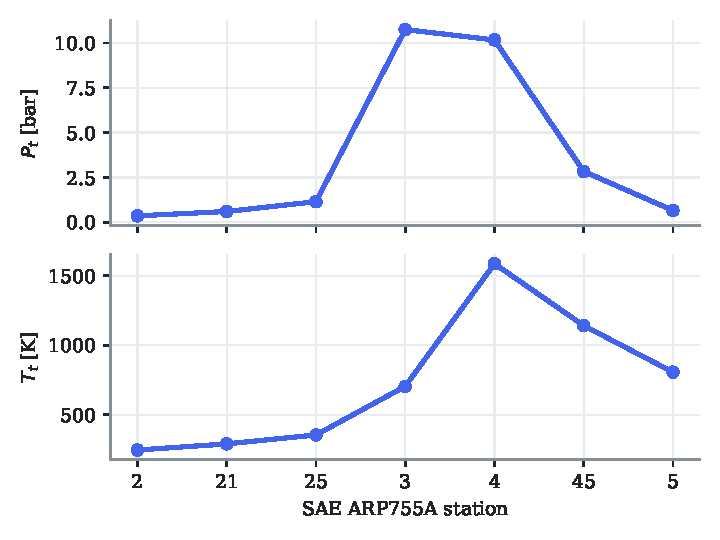
\includegraphics[width=0.72\textwidth]{design_stations}
  \caption{Total pressure and temperature along the gas path at the design point. Compression
  peaks at station 3 ($\sim$\SI{11}{bar}, \cref{tab:stations}), heat addition at station 4, and
  work extraction across stations 45 and 5.}
  \label{fig:stations}
\end{figure}

The design point converges with a Newton residual below $10^{-6}$ and satisfies all five
acceptance windows defined a priori: BPR $5.10\pm0.2$ (the EEDB target), OPR within its window,
$T_{t4}$ within a plausible band, total cooling-plus-bleed fraction between 18 and 25\,\% of
core flow, and thrust exactly on target (\cref{tab:design}). The resulting TSFC
($\approx0.62$~lb/(lbf$\cdot$h)) lands within 2\,\% of the publicly quoted cruise value for
this engine \emph{without having been used as a calibration target} ---an encouraging
consistency check.

\section{Calibration against measured data (WP1.2)}
\label{sec:calibration}

\subsection{Data sources and philosophy}

Off-design calibration uses exclusively \textbf{measured, certified data} (\cref{tab:tcds}).
The TCDS provides limits and rated thrusts. The ICAO Engine Emissions Databank provides
something less well known: sea-level test-bed \emph{measured fuel flows} at the four
landing-takeoff-cycle thrust settings (100, 85, 30 and 7\,\% of rated thrust $F_{00}$), plus
the engine pressure ratio at rated output (27.61) ---all for the exact -7B26 variant, traceable
to certification testing, and free. Most academic engine models ignore this source.

The anchor points are solved \emph{thrust-matched}: the fuel--air ratio balance is set to hold
$F_n = \mathrm{PC}\cdot F_{00}$ (PC being the power fraction). The model's fuel flow at each
anchor is therefore a genuine \textbf{prediction} confronted with the EEDB measurement ---not a
quantity fitted to it.

\subsection{Calibration iterations}

The first run (model freshly adapted from the example, not yet calibrated to the SLS data)
already predicted takeoff fuel flow within $-2.1$\,\%, but showed two quantitative defects:

\begin{enumerate}
  \item \textbf{N2 above its redline at rated thrust}: \SI{15311}{rpm} against the certified
    limit of \SI{15183}{rpm}. Cause: the reference speed used to scale the generic HPC map
    ---the map's speed-versus-flow shape is not the real compressor's, so the speed labels it
    implies must be anchored deliberately. Fix: HP-shaft design reference from \SI{14324}{} to
    \SI{13940}{rpm}, placing rated-thrust N2 at \SI{14915}{rpm} ($\approx103$\,\%), inside the
    limit.
  \item \textbf{Takeoff pressure ratio 28.99 versus the measured 27.61} ($+5.0$\,\%). Fix: HPC
    design pressure ratio from 9.81 to 9.35. The measured value takes precedence over the
    initial derived estimate, and the cruise OPR becomes a consequence ($\approx30$).
\end{enumerate}

\begin{table}[htbp]
  \centering\small
  \caption{SLS anchors versus the ICAO databank measurements after calibration. $W_f$~model is
  the model's prediction at imposed thrust. Auto-generated.}
  \label{tab:anchors}
  \input{tables/table_anchors}
\end{table}

\begin{figure}[htbp]
  \centering
  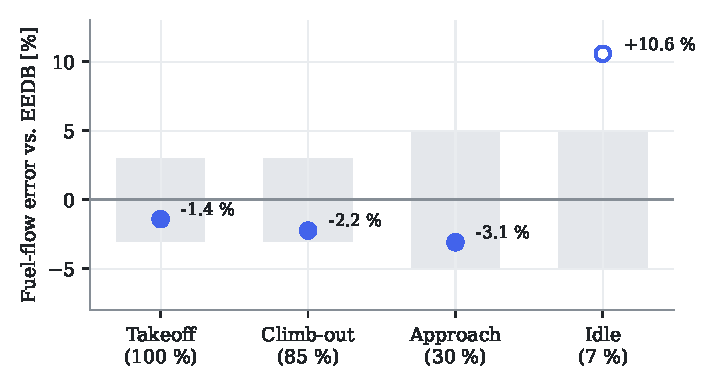
\includegraphics[width=0.7\textwidth]{anchor_errors}
  \caption{Fuel-flow prediction error at each anchor against the EEDB measurement. Gray bands
  are the contract tolerances ($\pm3$\,\% at takeoff and climb-out, $\pm5$\,\% at approach and
  idle); the hollow marker (idle) converges but sits outside tolerance and is reported without
  blocking the milestone (\cref{sec:idle}).}
  \label{fig:anchor-errors}
\end{figure}

\begin{figure}[htbp]
  \centering
  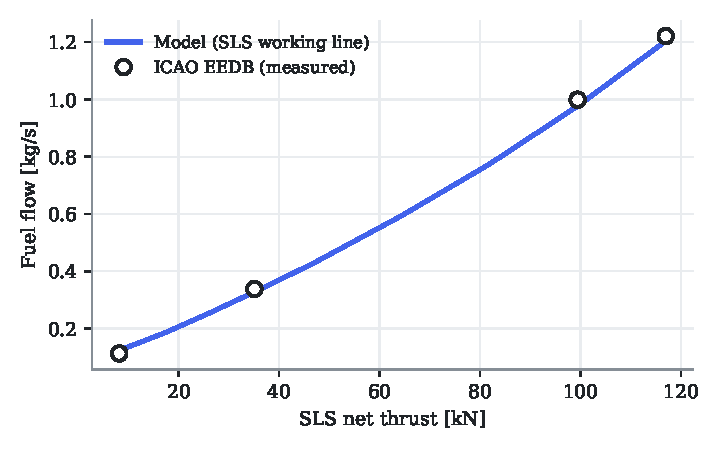
\includegraphics[width=0.7\textwidth]{sls_working_line}
  \caption{The model's sea-level-static working line (a continuous sweep of thrust setting)
  against the four measured ICAO databank points. The curvature at low power reflects the
  degraded accuracy of generic maps far from their scaling point.}
  \label{fig:working-line}
\end{figure}

After both corrections (\cref{tab:anchors,fig:anchor-errors,fig:working-line}), the three gated
anchors meet their tolerances: takeoff at $-1.40$\,\% fuel-flow error with the pressure ratio
within $+0.3$\,\% of the measured value and both shaft speeds inside their redlines; climb-out
at $-2.23$\,\%; approach at $-3.08$\,\%.

\subsection{Idle convergence: diagnosis and cure}
\label{sec:idle}

The idle point (7\,\% of $F_{00}$, static) systematically diverges from a cold start. At such
low power the nozzle pressure ratios approach unity ---the exhaust barely pushes--- and the
nozzles' internal static-pressure sub-solver bounces against its lower bound, leaving the
global Newton iteration without a descent direction. Worse, the failed attempt leaves the
point's internal states (flow stations, map positions) corrupted, so re-seeding only the
balance variables does not rescue it: the idle point must \emph{never} start cold at its final
setting. The cure ---anticipated as a generic countermeasure in the specification--- is
\textbf{power continuation}: the point starts at 30\,\% of $F_{00}$ (where it converges from
cold, just like the approach anchor) and walks down warm through
$0.30 \rightarrow 0.20 \rightarrow 0.14 \rightarrow 0.10 \rightarrow 0.08 \rightarrow 0.07$,
re-solving at each step. The logic is encapsulated in the library
(\code{solve\_anchors()}) and covered by the tests.

With continuation, idle converges and predicts fuel flow with $+10.6$\,\% error. This is deep
map-extrapolation territory ---the generic map's speed-flow shape at very low power is not the
real compressor's--- a known limitation of the approach; the anchor is \textbf{reported but not
gated} for milestone H1, a decision recorded in the calibration contract
(\code{gated:~false}).

\section{Baseline decks (WP1.3)}
\label{sec:decks}

Both EHM pipelines need a \emph{baseline}: what a healthy engine reads at any operating
condition, so that measured values can be turned into deviations. The baseline is produced by
sweeping the healthy model over a realistic flight envelope ---altitude blocks with their
plausible Mach ranges (no Mach~0.8 at sea level), ambient temperature offsets of 0, $+15$ and
$+30$\,\si{\degreeCelsius} above ISA, and six thrust settings from 50 to 100\,\% of the locally
available maximum. At each condition the model first finds the maximum thrust at the rating
temperature (point \code{OD\_max}, throttled by $T_{4}$), then solves the part-power point at
the commanded fraction (\code{OD\_pt}) ---the same two-point pattern used by the pyCycle
reference example.

Two engineering lessons from WP1.2 shaped the sweep. First, the walk is ordered for warm
starting within each block (thrust descending), and the independent (altitude, Mach) blocks run
in \emph{parallel processes}, one Problem per worker (project norm N1: long decomposable
computations are parallelized; the sweep takes $3.5$ minutes on all cores versus $10$ minutes
serial). Second ---the lesson learned the hard way--- a failed Newton attempt corrupts the
point's internal states beyond re-seeding, so the recovery action on any failure is to
\emph{rebuild} the problem cold with altitude-appropriate guesses (norm N2); a first version of
the sweep without this recovery lost every point downstream of the first divergence.

The result is stored as a table plus a scattered linear interpolator in the four operating
coordinates, and its quality is measured by leave-one-out cross-validation (each grid point
predicted from all the others), reported per channel in \cref{tab:deck-loo}. Median errors are
a few tenths of a percent; the tail percentiles are dominated by envelope-corner points whose
interpolation simplices span across altitude blocks in raw physical coordinates. This is
expected and temporary: the production baseline of phase F3 interpolates in
\emph{corrected-parameter} space (\cref{sec:stations}), where the $\theta$/$\delta$
normalization collapses most of the altitude and temperature dependence and the same grid is
far denser relative to the remaining variation.

\begin{table}[htbp]
  \centering\small
  \caption{Leave-one-out interpolation error of the baseline deck, per channel.
  Auto-generated.}
  \label{tab:deck-loo}
  % AUTOGENERATED by scripts/make_report_assets.py — do NOT edit by hand
\begin{tabular}{lrrr}
\toprule
Channel & Median [\%] & P95 [\%] & Max [\%] \\
\midrule
  Fuel flow & 0.498 & 15.767 & 90.603 \\
  N1 & 0.268 & 6.369 & 25.721 \\
  N2 & 0.080 & 2.649 & 9.697 \\
  EGT & 0.167 & 6.012 & 24.062 \\
  Net thrust & 0.000 & 16.437 & 85.402 \\
\bottomrule
\end{tabular}

\end{table}

\section{Influence coefficient matrix and observability (WP1.4)}
\label{sec:icm}

\subsection{Health-parameter injection}

To compute the ICM ---and, in phase F2, to simulate degraded engines--- the model must accept
imposed health deviations. pyCycle scales its generic component maps with per-component design
scalars (efficiency and flow); the off-design points normally inherit them from the design
point. In the \code{MPCFM56Study} model those connections are routed through multiplier
components, so that any efficiency or flow-capacity deviation can be dialed in per run. Two
implementation subtleties are worth recording: (i) the multipliers must execute \emph{before}
the off-design point ---the multi-point group runs its children in insertion order, and a
mis-ordered version silently solved the off-design point with unscaled maps; the symptom (a
``healthy'' point that did not reproduce the design point) was caught by the self-consistency
check below; and (ii) holding N1 constant, the CFM56's rating parameter, requires a fuel-flow
balance targeting the LP spool speed through a passthrough component, since the speed is itself
the output of another balance.

The wiring is validated by a self-consistency property that is now a permanent test: the
\emph{healthy} off-design point at cruise with N1 equal to its design value must reproduce the
design point exactly. It does: thrust \SI{5480.0}{lbf}, N2 \SI{13940.0}{rpm}, OPR 30.03, EGT
\SI{1141.6}{\kelvin} ---machine-precision agreement with \cref{tab:design}.

\subsection{The ICM at the reference conditions}

The ICM is computed by central finite differences ($\pm0.5$\,\% per health parameter) at the
two conditions where airline EHM snapshots are taken: cruise (M\,0.78/\SI{35000}{ft}) and
sea-level takeoff, at constant N1. \Cref{fig:icm} shows the cruise matrix for the extended
sensor set; every sign satisfies the physical expectations (e.g.\ a healthier HPT runs cooler
and thriftier: negative EGT and $W_f$ entries in its efficiency column), and these sign checks
run automatically in the test suite.

\begin{figure}[htbp]
  \centering
  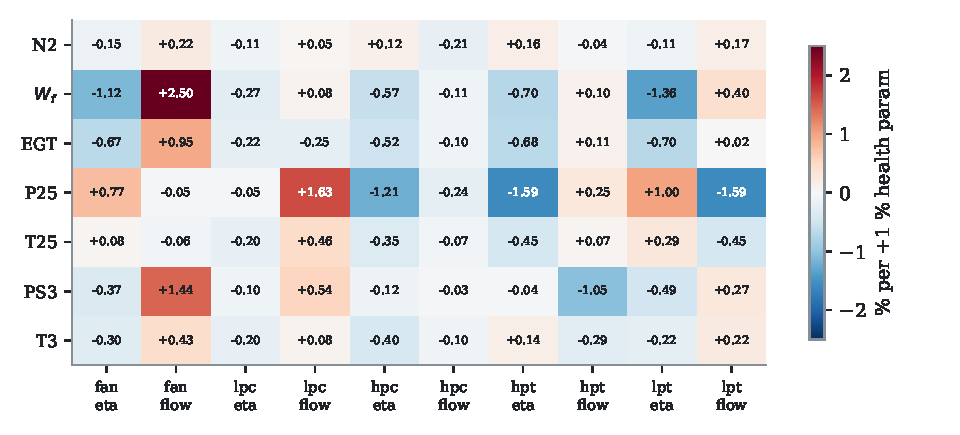
\includegraphics[width=\textwidth]{icm_cruise}
  \caption{Influence coefficient matrix at cruise (extended sensor set): \% change of each
  measured channel per $+1$\,\% change of each health parameter. Auto-generated from the
  model.}
  \label{fig:icm}
\end{figure}

\subsection{Observability: the quantitative case for hypothesis H2}

With the cockpit set only (N2, $W_f$, EGT ---N1 is the held rating parameter, so it carries no
information), the ICM has rank 3 for 10 unknowns and the geometry of its columns is damning:
the minimum angle between fault signatures is \textbf{1.3\,degrees}, with seven pairs below
15\,degrees (\cref{tab:confusable}). The most confusable pair, HPC efficiency versus HPT
efficiency, is precisely the classical HPC/HPT ambiguity reported in the GPA
literature~\cite{Li2002} ---here quantified for this engine. Two faults whose signatures differ
by 1.3\,degrees are, at realistic noise levels, indistinguishable to any linear
estimator: this is the smearing mechanism measured, and it defines the ``confusable'' subset on
which hypothesis H2 will compare the AI's isolation ability against WLS-GPA. The extended
sensor set (adding P25/T25/PS3/T3) raises the rank to 7 and multiplies the minimum angle by
roughly five ---the quantitative basis for the sensor-set ablation of contribution C6.

\begin{table}[htbp]
  \centering\small
  \caption{Confusable fault pairs at cruise with cockpit sensors (signature angle
  $<15^{\circ}$). Auto-generated.}
  \label{tab:confusable}
  % AUTOGENERATED by scripts/make_report_assets.py — do NOT edit by hand
\begin{tabular}{llr}
\toprule
Fault A & Fault B & Angle [deg] \\
\midrule
  $\eta_{\mathrm{HPC}}$ & $\eta_{\mathrm{HPT}}$ & 1.32 \\
  $\eta_{\mathrm{FAN}}$ & $\eta_{\mathrm{LPT}}$ & 4.32 \\
  $\eta_{\mathrm{HPT}}$ & $\Gamma_{\mathrm{HPT}}$ & 6.02 \\
  $\Gamma_{\mathrm{FAN}}$ & $\eta_{\mathrm{LPT}}$ & 6.52 \\
  $\eta_{\mathrm{HPC}}$ & $\Gamma_{\mathrm{HPT}}$ & 7.20 \\
  $\eta_{\mathrm{FAN}}$ & $\Gamma_{\mathrm{FAN}}$ & 10.05 \\
  $\eta_{\mathrm{FAN}}$ & $\eta_{\mathrm{LPC}}$ & 13.53 \\
\bottomrule
\end{tabular}

\end{table}

\subsection{Thermodynamics cross-check}

Decision D2 (tabular thermodynamics for speed) is closed by re-solving the design point with
NASA's chemical-equilibrium code (CEA): all key quantities agree within
0.7\,\% (\cref{tab:cea}), an order of magnitude below the $\pm3$\,\% calibration tolerance.
Tabular thermodynamics is therefore retained for all fleet-scale computation.

\begin{table}[htbp]
  \centering\small
  \caption{Design point solved with tabular versus CEA thermodynamics. Auto-generated.}
  \label{tab:cea}
  % AUTOGENERATED by scripts/make_report_assets.py — do NOT edit by hand
\begin{tabular}{lrrr}
\toprule
Quantity & Tabular & CEA & $\Delta$ [\%] \\
\midrule
  Net thrust [lbf] & 5480.0000 & 5480.0000 & -0.000 \\
  TSFC [lb/(lbf$\cdot$h)] & 0.6214 & 0.6249 & +0.553 \\
  Inlet mass flow [lbm/s] & 313.0851 & 315.2029 & +0.676 \\
  Fuel--air ratio & 0.0251 & 0.0250 & -0.122 \\
  HPT expansion ratio & 3.5865 & 3.5902 & +0.104 \\
  LPT expansion ratio & 4.2879 & 4.3109 & +0.537 \\
\bottomrule
\end{tabular}

\end{table}

\section{Declared limitations}
\label{sec:limitations}

The model is \emph{representative}, not certifiable, and its limits are declared for citation
in the results chapters: (i) no transients ---steady-state points only; (ii) variable geometry
(bleed valves, variable stators) implicit in the maps, not modeled; (iii) no Reynolds or
humidity corrections; (iv) absolute N1/N2 labels approximate by construction (generic map
shapes), though respecting the certified redlines at the rated point; (v) the model's EGT is
the HPT-exit temperature (station 45), a consistent proxy ---identical for ground truth and for
both EHM pipelines--- of the certified T49.5, whose displayed value additionally carries the
shunt and trim functions described in \cref{sec:engine}; and (vi) the idle error quoted above.
None of these limitations affects the validity of the AI-versus-traditional comparison, which
rests on the model's sensitivity structure (the ICM), not on its absolute values.

\section{Automated verification}

The chapter's claims are pinned by tests: design-point convergence and acceptance windows;
convergence of all four anchors including the idle continuation; fuel-flow and pressure-ratio
tolerances at the gated anchors; N1/N2 redlines at rated thrust; the Study self-consistency
property (healthy off-design $=$ design); the ICM physical sign checks and its rank-3 cockpit
underdetermination; and the pyCycle environment smoke test. Twelve tests green in continuous
integration at the time of writing.

\chapter{Work in progress and planning}
\label{ch:wip}

\section{Closing phase F1}

WP1.3 (baseline decks) and WP1.4 (influence coefficient matrix, observability analysis and
thermodynamics cross-check) are documented in \cref{sec:decks,sec:icm}. Remaining before
declaring H1 closed: extending the ICM to a grid of operating conditions (currently the two
snapshot reference conditions), the corrected-parameter exponent regressions on the deck, and
densifying the deck grid wherever the leave-one-out error concentrates.

\section{Remaining phases}

\begin{table}[htbp]
  \centering\small
  \caption{Remaining phases, key deliverables and closing criteria.}
  \label{tab:remaining-phases}
  \begin{tabular}{p{1.2cm}p{5.6cm}p{6.6cm}}
    \toprule
    Phase & Key deliverable & Closing criterion (gate) \\
    \midrule
    F2 & SynCFM56 v1.0: synthetic fleet of $\sim$100 engines with ground truth and ACARS-style
         snapshots &
         H2: realism and difficulty audit passed; no leakage between splits; dataset datasheet
         written \\
    F3 & Complete traditional pipeline (baseline, trending, WLS, Kalman, rules, extrapolation
         RUL) &
         H3: full metrics on test; smearing measured against ground truth \\
    F4 & AI suite (detection, diagnosis, RUL, physics-informed hybrid, conformal intervals,
         PCS) &
         H4: beats the traditional pipeline on $\geq1$ primary metric per task on validation \\
    F5 & Pre-registered evaluation + ablations + N-CMAPSS &
         H5: hypotheses H1--H5 resolved with statistical tests; figures reproducible with one
         command \\
    F6 & Case studies, dashboard, final report &
         H6: full reproduction from raw data; defensible document \\
    \bottomrule
  \end{tabular}
\end{table}

\section{Milestone log}

\begin{table}[htbp]
  \centering\small
  \caption{Milestones reached (updated at every gate).}
  \label{tab:milestone-log}
  \begin{tabular}{llp{8.6cm}}
    \toprule
    Milestone & Date & Evidence \\
    \midrule
    H0 & 2026-07-03 & Reproducible environment (uv, Python 3.11, pyCycle 4.4 with
      \code{numpy<2}); a complete example cycle converging locally and in CI; repository
      skeleton and smoke test. \\
    H1 (partial) & 2026-07-03 & WP1.1 and WP1.2 complete: design point inside all five
      acceptance windows (\cref{tab:design}); SLS anchors calibrated against TCDS + EEDB with
      all three gated anchors in tolerance (\cref{tab:anchors}); calibration contract with
      verified values. \\
    H1 (WP1.3--1.4) & 2026-07-03 & Baseline decks over the flight envelope with leave-one-out
      quality report (\cref{tab:deck-loo}); health-parameter injection validated by the
      off-design/design self-consistency check; ICM at both snapshot conditions with SVD
      observability analysis --- minimum cockpit signature angle 1.3$^{\circ}$, seven
      confusable pairs (\cref{tab:confusable}); tabular-vs-CEA cross-check within 0.7\,\%
      (\cref{tab:cea}); twelve automated tests green. \\
    \bottomrule
  \end{tabular}
\end{table}


\printbibliography[heading=bibintoc,title={References}]

\end{document}
